\documentclass[varwidth=6.2in,border=3pt]{standalone}
\usepackage{tikz}
\usetikzlibrary{arrows.meta,decorations.pathreplacing,positioning,calc,fit}
\usepackage{amsmath}
\usepackage{algpseudocode}
\usepackage{newtxtext,newtxmath}
\newcommand{\code}[1]{\texttt{#1}}
\newcommand{\truesum}{\code{truesum}}
\begin{document}
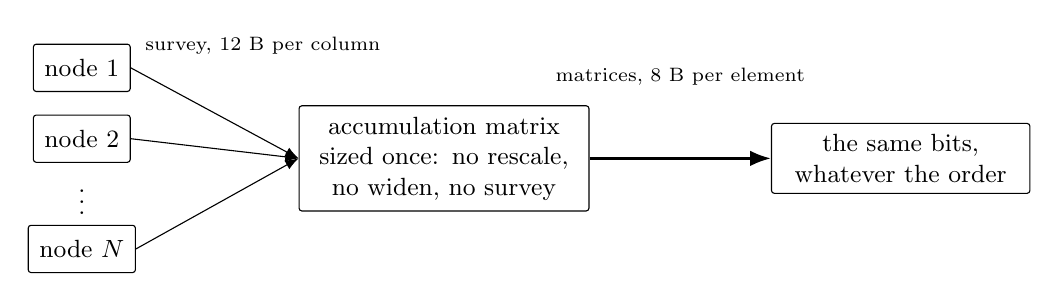
\begin{tikzpicture}[font=\small,
  box/.style={draw,rounded corners=1pt,inner sep=4pt,minimum height=6mm},
  arr/.style={-Latex}]
  % Producers on the left, each sending only its survey.
  \node[box] (n1) at (0,1.5) {node 1};
  \node[box] (n2) at (0,0.6) {node 2};
  \node at (0,-0.1) {$\vdots$};
  \node[box] (nN) at (0,-0.8) {node $N$};
  % The accumulation matrix, sized once from all of them.
  \node[box,text width=34mm,align=center] (acc) at (4.6,0.35)
    {accumulation matrix\\sized once: no rescale,\\no widen, no survey};
  \foreach \s in {n1,n2,nN} { \draw[arr] (\s.east) -- (acc.west); }
  \node[font=\scriptsize,anchor=south] at (2.3,1.55) {survey, 12 B per column};
  % Then the data itself, in any order.
  \node[box,text width=30mm,align=center] (out) at (10.4,0.35)
    {the same bits,\\whatever the order};
  \draw[arr,line width=1pt] (acc.east)
    -- node[font=\scriptsize,above=8mm,midway] {matrices, 8 B per element} (out.west);
\end{tikzpicture}
\end{document}
